% !TEX root = Apostila GP.tex

\capitulo{Tempo}

Para gerenciramos o tempo, é preciso primeiramente termos o escopo bem definido, pois o último é base para o primeiro.

\section{Definir atividades}

A partir da EAP vamos traçar a fronteira entre o escopo e o tempo. Isso é feito através da definição das atividades.

Escopo é \textbf{o que} o projeto vai entregar. As atividades são o \textbf{como}, ou seja, de que forma o projeto vai realizar as entregas. A Tabela \ref{tab:ativ:ex} traz alguns exemplos de atividades associadas ao escopo.

\begin{table}[h!]\footnotesize
\centering
\begin{tabular}
{
 	|p{1,8cm}
	| >{\centering\arraybackslash}p{4,9cm}|
}

	\hline

	\multicolumn{2}{c}{Projeto ``Cadeira''}\\
	
	\hline
	
	Escopo&
	Atividade\\
	
	\hline

	Braço&
	\begin{itemize}
		\item Cortar madeira
		\item Lixar
		\item Colar
		\item Envernizar
	\end{itemize}\\
	
	\hline

	Assento&
	\begin{itemize}
		\item Cortar pano
		\item Cortar espuma
		\item Costurar
	\end{itemize}\\

	\hline

\end{tabular}
\caption {Exemplo de lista de atividades}
\label{tab:ativ:ex}
\end{table}

\section{Sequenciar atividades}

Sequenciar é definir a ordem e também as dependências das atividades.

\section{Estimar os recursos das atividades}

Quais os recursos materiais, humanos e tecnológicos que serão necessários para executar cada uma das atividades?

\section{Estimar as durações das atividades}

Quanto tempo será necessário para se concluir cada uma das atividades?

\section{Desenvolver o cronograma}

Um cronograma deve conter:

\begin{itemize}

\item A EAP associada à lista de atividades;

\item O sequenciamento das atividades;

\item Os recursos estimados;

\item As durações estimadas das atividades;

\item As datas reais de início e fim das atividades.

\end{itemize}

A Figura \ref{fig:ativ:ex} traz um exemplo de crongrama contendo todos os elementos citados acima.

\begin{figure}[!h]
\centering
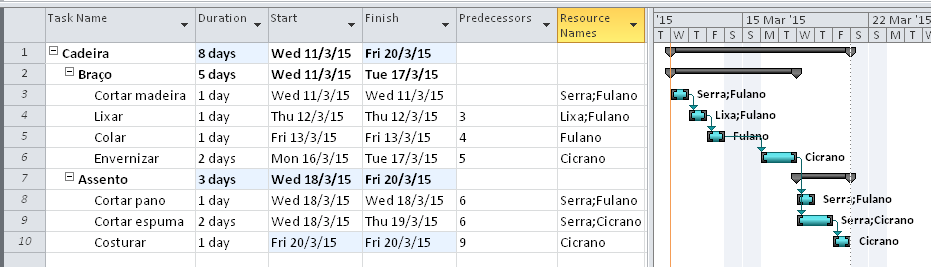
\includegraphics[scale=0.45]{Figuras/ativ_exemplo.png}
\caption{Exemplo de cronograma}
\label{fig:ativ:ex}
\end{figure}